
%% bare_conf.tex
%% V1.4
%% 2012/12/27
%% by Michael Shell
%% See:
%% http://www.michaelshell.org/
%% for current contact information.
%%
%% This is a skeleton file demonstrating the use of IEEEtran.cls
%% (requires IEEEtran.cls version 1.8 or later) with an IEEE conference paper.
%%
%% Support sites:
%% http://www.michaelshell.org/tex/ieeetran/
%% http://www.ctan.org/tex-archive/macros/latex/contrib/IEEEtran/
%% and
%% http://www.ieee.org/

%%*************************************************************************
%% Legal Notice:
%% This code is offered as-is without any warranty either expressed or
%% implied; without even the implied warranty of MERCHANTABILITY or
%% FITNESS FOR A PARTICULAR PURPOSE! 
%% User assumes all risk.
%% In no event shall IEEE or any contributor to this code be liable for
%% any damages or losses, including, but not limited to, incidental,
%% consequential, or any other damages, resulting from the use or misuse
%% of any information contained here.
%%
%% All comments are the opinions of their respective authors and are not
%% necessarily endorsed by the IEEE.
%%
%% This work is distributed under the LaTeX Project Public License (LPPL)
%% ( http://www.latex-project.org/ ) version 1.3, and may be freely used,
%% distributed and modified. A copy of the LPPL, version 1.3, is included
%% in the base LaTeX documentation of all distributions of LaTeX released
%% 2003/12/01 or later.
%% Retain all contribution notices and credits.
%% ** Modified files should be clearly indicated as such, including  **
%% ** renaming them and changing author support contact information. **
%%
%% File list of work: IEEEtran.cls, IEEEtran_HOWTO.pdf, bare_adv.tex,
%%                    bare_conf.tex, bare_jrnl.tex, bare_jrnl_compsoc.tex,
%%                    bare_jrnl_transmag.tex
%%*************************************************************************

% *** Authors should verify (and, if needed, correct) their LaTeX system  ***
% *** with the testflow diagnostic prior to trusting their LaTeX platform ***
% *** with production work. IEEE's font choices can trigger bugs that do  ***
% *** not appear when using other class files.                            ***
% The testflow support page is at:
% http://www.michaelshell.org/tex/testflow/



% Note that the a4paper option is mainly intended so that authors in
% countries using A4 can easily print to A4 and see how their papers will
% look in print - the typesetting of the document will not typically be
% affected with changes in paper size (but the bottom and side margins will).
% Use the testflow package mentioned above to verify correct handling of
% both paper sizes by the user's LaTeX system.
%
% Also note that the "draftcls" or "draftclsnofoot", not "draft", option
% should be used if it is desired that the figures are to be displayed in
% draft mode.
%
\documentclass[conference]{IEEEtran}
% Add the compsoc option for Computer Society conferences.
%
% If IEEEtran.cls has not been installed into the LaTeX system files,
% manually specify the path to it like:
% \documentclass[conference]{../sty/IEEEtran}





% Some very useful LaTeX packages include:
% (uncomment the ones you want to load)


% *** MISC UTILITY PACKAGES ***
%
%\usepackage{ifpdf}
% Heiko Oberdiek's ifpdf.sty is very useful if you need conditional
% compilation based on whether the output is pdf or dvi.
% usage:
% \ifpdf
%   % pdf code
% \else
%   % dvi code
% \fi
% The latest version of ifpdf.sty can be obtained from:
% http://www.ctan.org/tex-archive/macros/latex/contrib/oberdiek/
% Also, note that IEEEtran.cls V1.7 and later provides a builtin
% \ifCLASSINFOpdf conditional that works the same way.
% When switching from latex to pdflatex and vice-versa, the compiler may
% have to be run twice to clear warning/error messages.






% *** CITATION PACKAGES ***
%
%\usepackage{cite}
% cite.sty was written by Donald Arseneau
% V1.6 and later of IEEEtran pre-defines the format of the cite.sty package
% \cite{} output to follow that of IEEE. Loading the cite package will
% result in citation numbers being automatically sorted and properly
% "compressed/ranged". e.g., [1], [9], [2], [7], [5], [6] without using
% cite.sty will become [1], [2], [5]--[7], [9] using cite.sty. cite.sty's
% \cite will automatically add leading space, if needed. Use cite.sty's
% noadjust option (cite.sty V3.8 and later) if you want to turn this off
% such as if a citation ever needs to be enclosed in parenthesis.
% cite.sty is already installed on most LaTeX systems. Be sure and use
% version 4.0 (2003-05-27) and later if using hyperref.sty. cite.sty does
% not currently provide for hyperlinked citations.
% The latest version can be obtained at:
% http://www.ctan.org/tex-archive/macros/latex/contrib/cite/
% The documentation is contained in the cite.sty file itself.






% *** GRAPHICS RELATED PACKAGES ***
%
\ifCLASSINFOpdf
  % \usepackage[pdftex]{graphicx}
  % declare the path(s) where your graphic files are
  % \graphicspath{{../pdf/}{../jpeg/}}
  % and their extensions so you won't have to specify these with
  % every instance of \includegraphics
  % \DeclareGraphicsExtensions{.pdf,.jpeg,.png}
\else
  % or other class option (dvipsone, dvipdf, if not using dvips). graphicx
  % will default to the driver specified in the system graphics.cfg if no
  % driver is specified.
  % \usepackage[dvips]{graphicx}
  % declare the path(s) where your graphic files are
  % \graphicspath{{../eps/}}
  % and their extensions so you won't have to specify these with
  % every instance of \includegraphics
  % \DeclareGraphicsExtensions{.eps}
\fi
% graphicx was written by David Carlisle and Sebastian Rahtz. It is
% required if you want graphics, photos, etc. graphicx.sty is already
% installed on most LaTeX systems. The latest version and documentation
% can be obtained at: 
% http://www.ctan.org/tex-archive/macros/latex/required/graphics/
% Another good source of documentation is "Using Imported Graphics in
% LaTeX2e" by Keith Reckdahl which can be found at:
% http://www.ctan.org/tex-archive/info/epslatex/
%
% latex, and pdflatex in dvi mode, support graphics in encapsulated
% postscript (.eps) format. pdflatex in pdf mode supports graphics
% in .pdf, .jpeg, .png and .mps (metapost) formats. Users should ensure
% that all non-photo figures use a vector format (.eps, .pdf, .mps) and
% not a bitmapped formats (.jpeg, .png). IEEE frowns on bitmapped formats
% which can result in "jaggedy"/blurry rendering of lines and letters as
% well as large increases in file sizes.
%
% You can find documentation about the pdfTeX application at:
% http://www.tug.org/applications/pdftex





% *** MATH PACKAGES ***
%
%\usepackage[cmex10]{amsmath}
% A popular package from the American Mathematical Society that provides
% many useful and powerful commands for dealing with mathematics. If using
% it, be sure to load this package with the cmex10 option to ensure that
% only type 1 fonts will utilized at all point sizes. Without this option,
% it is possible that some math symbols, particularly those within
% footnotes, will be rendered in bitmap form which will result in a
% document that can not be IEEE Xplore compliant!
%
% Also, note that the amsmath package sets \interdisplaylinepenalty to 10000
% thus preventing page breaks from occurring within multiline equations. Use:
%\interdisplaylinepenalty=2500
% after loading amsmath to restore such page breaks as IEEEtran.cls normally
% does. amsmath.sty is already installed on most LaTeX systems. The latest
% version and documentation can be obtained at:
% http://www.ctan.org/tex-archive/macros/latex/required/amslatex/math/





% *** SPECIALIZED LIST PACKAGES ***
%
%\usepackage{algorithmic}
% algorithmic.sty was written by Peter Williams and Rogerio Brito.
% This package provides an algorithmic environment fo describing algorithms.
% You can use the algorithmic environment in-text or within a figure
% environment to provide for a floating algorithm. Do NOT use the algorithm
% floating environment provided by algorithm.sty (by the same authors) or
% algorithm2e.sty (by Christophe Fiorio) as IEEE does not use dedicated
% algorithm float types and packages that provide these will not provide
% correct IEEE style captions. The latest version and documentation of
% algorithmic.sty can be obtained at:
% http://www.ctan.org/tex-archive/macros/latex/contrib/algorithms/
% There is also a support site at:
% http://algorithms.berlios.de/index.html
% Also of interest may be the (relatively newer and more customizable)
% algorithmicx.sty package by Szasz Janos:
% http://www.ctan.org/tex-archive/macros/latex/contrib/algorithmicx/




% *** ALIGNMENT PACKAGES ***
%
%\usepackage{array}
% Frank Mittelbach's and David Carlisle's array.sty patches and improves
% the standard LaTeX2e array and tabular environments to provide better
% appearance and additional user controls. As the default LaTeX2e table
% generation code is lacking to the point of almost being broken with
% respect to the quality of the end results, all users are strongly
% advised to use an enhanced (at the very least that provided by array.sty)
% set of table tools. array.sty is already installed on most systems. The
% latest version and documentation can be obtained at:
% http://www.ctan.org/tex-archive/macros/latex/required/tools/


% IEEEtran contains the IEEEeqnarray family of commands that can be used to
% generate multiline equations as well as matrices, tables, etc., of high
% quality.




% *** SUBFIGURE PACKAGES ***
%\ifCLASSOPTIONcompsoc
%  \usepackage[caption=false,font=normalsize,labelfont=sf,textfont=sf]{subfig}
%\else
%  \usepackage[caption=false,font=footnotesize]{subfig}
%\fi
% subfig.sty, written by Steven Douglas Cochran, is the modern replacement
% for subfigure.sty, the latter of which is no longer maintained and is
% incompatible with some LaTeX packages including fixltx2e. However,
% subfig.sty requires and automatically loads Axel Sommerfeldt's caption.sty
% which will override IEEEtran.cls' handling of captions and this will result
% in non-IEEE style figure/table captions. To prevent this problem, be sure
% and invoke subfig.sty's "caption=false" package option (available since
% subfig.sty version 1.3, 2005/06/28) as this is will preserve IEEEtran.cls
% handling of captions.
% Note that the Computer Society format requires a larger sans serif font
% than the serif footnote size font used in traditional IEEE formatting
% and thus the need to invoke different subfig.sty package options depending
% on whether compsoc mode has been enabled.
%
% The latest version and documentation of subfig.sty can be obtained at:
% http://www.ctan.org/tex-archive/macros/latex/contrib/subfig/




% *** FLOAT PACKAGES ***
%
%\usepackage{fixltx2e}
% fixltx2e, the successor to the earlier fix2col.sty, was written by
% Frank Mittelbach and David Carlisle. This package corrects a few problems
% in the LaTeX2e kernel, the most notable of which is that in current
% LaTeX2e releases, the ordering of single and double column floats is not
% guaranteed to be preserved. Thus, an unpatched LaTeX2e can allow a
% single column figure to be placed prior to an earlier double column
% figure. The latest version and documentation can be found at:
% http://www.ctan.org/tex-archive/macros/latex/base/


%\usepackage{stfloats}
% stfloats.sty was written by Sigitas Tolusis. This package gives LaTeX2e
% the ability to do double column floats at the bottom of the page as well
% as the top. (e.g., "\begin{figure*}[!b]" is not normally possible in
% LaTeX2e). It also provides a command:
%\fnbelowfloat
% to enable the placement of footnotes below bottom floats (the standard
% LaTeX2e kernel puts them above bottom floats). This is an invasive package
% which rewrites many portions of the LaTeX2e float routines. It may not work
% with other packages that modify the LaTeX2e float routines. The latest
% version and documentation can be obtained at:
% http://www.ctan.org/tex-archive/macros/latex/contrib/sttools/
% Do not use the stfloats baselinefloat ability as IEEE does not allow
% \baselineskip to stretch. Authors submitting work to the IEEE should note
% that IEEE rarely uses double column equations and that authors should try
% to avoid such use. Do not be tempted to use the cuted.sty or midfloat.sty
% packages (also by Sigitas Tolusis) as IEEE does not format its papers in
% such ways.
% Do not attempt to use stfloats with fixltx2e as they are incompatible.
% Instead, use Morten Hogholm'a dblfloatfix which combines the features
% of both fixltx2e and stfloats:
%
% \usepackage{dblfloatfix}
% The latest version can be found at:
% http://www.ctan.org/tex-archive/macros/latex/contrib/dblfloatfix/




% *** PDF, URL AND HYPERLINK PACKAGES ***
%
%\usepackage{url}
% url.sty was written by Donald Arseneau. It provides better support for
% handling and breaking URLs. url.sty is already installed on most LaTeX
% systems. The latest version and documentation can be obtained at:
% http://www.ctan.org/tex-archive/macros/latex/contrib/url/
% Basically, \url{my_url_here}.




% *** Do not adjust lengths that control margins, column widths, etc. ***
% *** Do not use packages that alter fonts (such as pslatex).         ***
% There should be no need to do such things with IEEEtran.cls V1.6 and later.
% (Unless specifically asked to do so by the journal or conference you plan
% to submit to, of course. )


% correct bad hyphenation here
\hyphenation{op-tical net-works semi-conduc-tor}
\usepackage{graphicx}% http://ctan.org/pkg/graphicx
\usepackage{multirow}% http://ctan.org/pkg/multirow
\usepackage{booktabs}% http://ctan.org/pkg/booktabs
\usepackage{float}
\usepackage{tabularx,booktabs}
\graphicspath{{images/}}
\usepackage[export]{adjustbox}
\usepackage{siunitx}
\usepackage{etoolbox}
\newcommand\mcbf[1]{\multicolumn{1}{>{\centering\arraybackslash\bfseries}X}{#1}}
\newrobustcmd{\B}{\fontseries{b}\selectfont} % non-extended bold font
\usepackage{hyperref}
\begin{document}
%
% paper title
% can use linebreaks \\ within to get better formatting as desired
% Do not put math or special symbols in the title.
\title{Comparing approaches to analyze sentiment}


% author names and affiliations
% use a multiple column layout for up to three different
% affiliations
\author{\IEEEauthorblockN{Luka Žontar}
\IEEEauthorblockA{Faculty of Computer and Information Science\\
University of Ljubljana\\
Ljubljana, Slovenia\\
Email: lz3057@student.uni-lj.si}}
% conference papers do not typically use \thanks and this command
% is locked out in conference mode. If really needed, such as for
% the acknowledgment of grants, issue a \IEEEoverridecommandlockouts
% after \documentclass

% for over three affiliations, or if they all won't fit within the width
% of the page, use this alternative format:
% 
%\author{\IEEEauthorblockN{Michael Shell\IEEEauthorrefmark{1},
%Homer Simpson\IEEEauthorrefmark{2},
%James Kirk\IEEEauthorrefmark{3}, 
%Montgomery Scott\IEEEauthorrefmark{3} and
%Eldon Tyrell\IEEEauthorrefmark{4}}
%\IEEEauthorblockA{\IEEEauthorrefmark{1}School of Electrical and Computer Engineering\\
%Georgia Institute of Technology,
%Atlanta, Georgia 30332--0250\\ Email: see http://www.michaelshell.org/contact.html}
%\IEEEauthorblockA{\IEEEauthorrefmark{2}Twentieth Century Fox, Springfield, USA\\
%Email: homer@thesimpsons.com}
%\IEEEauthorblockA{\IEEEauthorrefmark{3}Starfleet Academy, San Francisco, California 96678-2391\\
%Telephone: (800) 555--1212, Fax: (888) 555--1212}
%\IEEEauthorblockA{\IEEEauthorrefmark{4}Tyrell Inc., 123 Replicant Street, Los Angeles, California 90210--4321}}




% use for special paper notices
%\IEEEspecialpapernotice{(Invited Paper)}




% make the title area
\maketitle

% As a general rule, do not put math, special symbols or citations
% in the abstract
\begin{abstract}
Sentiment analysis can help us automatically determine writer's attitude towards the text on enormous datasets. In practice, it helps companies make important business decisions and evaluate public opinions on their products. This article should help readers understand different machine learning approaches to sentiment analysis. We also explain how textual data should be preprocessed generally and for different models. 

This article focuses on deep learning machine learning models. At first, we take the Naive Bayesian model to compare it with more complex machine learning  learning models. In particular, we try to evaluate a deep neural network with LSTM architecture and a BERT model that was fine-tuned on data that was used in training and validationof other models. As our dataset, we used Sentiment140, which contains pre-classified Twitter posts. In the end, we combine the aforementioned models to construct a majority voting ensemble model.


\end{abstract}

\begin{IEEEkeywords}
Sentiment analysis; classification; deep learning; neural networks.
\end{IEEEkeywords}




% For peer review papers, you can put extra information on the cover
% page as needed:
% \ifCLASSOPTIONpeerreview
% \begin{center} \bfseries EDICS Category: 3-BBND \end{center}
% \fi
%
% For peerreview papers, this IEEEtran command inserts a page break and
% creates the second title. It will be ignored for other modes.
\IEEEpeerreviewmaketitle



\section{Introduction}
Sentiment analysis is becoming an important technique used in many companies worldwide. With it, we use natural language processing to systematically identify subjectiveness in texts. In other words, in sentiment analysis we try to determine, whether the writer is positively or negatively affected by the written content. 
We try to evaluate writer's inclination towards the text using natural language processing and machine learning techniques to assign sentiment scores to phrases and sentences.  

In practice, sentiment analysis helps us automatically process enormous amounts of textual data that customers write on social media and in survey responses. Customer feedback analysis can help us determine whether or not customers are happy with our product. This can improve our company's strategic decisions, such as deciding in which product to invest or how to make customers happier.

Furthermore, it can help better understand public opinions about a particular subject. This can help politics predicting voting results and consequently form alliances between parties. Understanding people's opionions can also make us better investors, since stock market stability depends on other investors.

 which can help us predicting voting results or even stock market state. 

In this article, we focus on comparing different sentiment analysis techniques. The goal of this article is to help readers understand different types of sentiment analysis approaches and when they should be used. We explain different preprocessing techniques and compare a baseline Naive Bayesian model with more complex deep learning based models LSTM and BERT. In the end, we compare results with a majority voting ensemble model that is combined of all three aforementioned models. 

For learning and validation we use the Sentiment140 dataset, which contains pre-classified Twitter posts. Tweets represent the general public and thus all sorts of opinions can be found in the dataset we used. Some opinions are stronger and in some it is difficult to determine the writer's inclination towards the text topic. This makes the given dataset an appropriate training and validation set.

In next section, we make an overview of related work that was relevant for our research. After that, we explain the methodology of our work, that is, how data was preprocessed and how models were evaluated. In the forth and fifth section, we present results and discuss them. Lastly, we conclude this article by presenting the main findings.

\section{Related work}
In this section, we present related work that was relevant for our article. Sentiment analysis was proven to be useful in different areas. For example, in medicine, sentiment analysis is used to evaluate healthcare textual data. In medical sentiment, we use medical information to achieve the best result to increase healthcare quality \cite{DENECKE201517}. As mentioned before, social media holds loads of textual data of different sorts. Muzafar et al. discusesed how SARS-Cov-2 affected people on social media \cite{covid19}. At first, the most commonly searched terms were Coronavirus related. And lots of negativity could be seen textual data from social media. 

Feldman \cite{feldman} discusses several approaches of sentiment analysis based on the basic unit that we will be classifying. We can classify whole documents, sentences or even particular aspects. Furthermore, we have to consider comparative statements such as less and more. As the most crucial field of sentiment analysis Feldman states sentiment lexicon acquisition, where words can be expanded in a set of words using corpus-based approaches or WordNet.

In past works, lots of researchers also worked on textual data preprocessing. Magliani and his colleauges \cite{magliani} evaluated lots of preprocessing techniques and found that preprocessing vastly increases model's accuracy. However, they found that basic preprocessing with stemming is the best way to improve accuracy with preprocessing. They also found that processing negations, stopwords and emoticons also slightly increases accuracy.

Latha \cite{latha} focused on how to process informal social media texts and emphasized the importance of removing URLs, special characters and repeated letters from texts. Furthermore, she proposed that question words should be removed from texts. We also noticed an interesting approach by Krouska et al. \cite{krouska}, who focused on the length of n-grams passed to classifiers. N-grams of length greater than 1 hold a lot more information about the text polarity than a single word, which is why they are used to get better accuracy on sentiment analysis classification.

To better understand sentiment analysis, we also need to get acquainted with the top performing machine learning models. Zainudin \cite{zainudin} split the sentiment analysis models into three major categories, lexicon based, machine learning based and hybrid approaches. Machine learning based approaches are further devided into supervised, semi-supervised and unsupervised approaches. In this article, we will be focusing on supervised machine learning approaches.

Starting with simpler methods, Dey \cite{naivebayes} et al. used statistical models to capture elements of subjective style and the sentence polarity. They managed to get above 80\% accuracy on a movie review dataset that is comprised of 4500 samples. In this study, Naive Bayesian classifier was compared with k-NN classifier. However, k-NN classifier failed to achieve comparable results on this dataset. Researchers also noticed high discrepancies amongst accuracies on different datasets.

In recent years, there have been several breakthroughs in the area of sentiment analysis. Recurrent neural network architectures, such as long short-term memory (LSTM), have proven to be very succesful in learning to evaluate polarity of text. Besides the standard feedforward connections, LSTM adds feedback connections. Putra et al. \cite{lstm} improved the basic LSTM architecture by adding exploiting the use of Word2Vec embeddings. They managed to achieve 85.96\% accuracy. Word embeddings make the regular LSTM architecture more robust to overfitting. For Arabic texts, an additional improvement to LSTM architecture was proposed by Elfaik and Nfaoui \cite{bilstm}, who used a deep bidirectional LSTM network to further increase the accuracy. While the complex model clearly overfitted on some datasets, it reached over 90\% accuracy on others.

A novel approach was proposed by Devlin and colleauges \cite{devlin2019bert}, who used deep bidirectional transformers for language understanding. These transformers were trained on enormous datasets and finally fine-tuned on sentiment analysis tasks to produce state-of-the-art results. 

\section{Methods}
In this section, we explain different methods that were used in this comparative study. Firstly, we describe the data that we used to get our results. Next, we explain the preprocessing methodology and finally, we describe the machine learning models that were used in this research. We used four different models: Naive Bayesian classifier, neural network with deep bidirectional LSTM architecture, BERT model fine-tuned with our data and a majority voting ensemble classifier.

\subsection{Data}
As already mentioned, we decided to use the \href{https://www.kaggle.com/kazanova/sentiment140}{Sentiment140 dataset} that contains 1,600,000 tweets extracted using Twitter API. In Figure \ref{pic1} we can see the most common words in the wordcloud representation. Due to time complexity of our research, we only use a randomly sampled subset of 40,000 tweets. While the dataset holds multiple features, we only use the tweet text and target variable from which we filter out the neutral tweets to make our problem a binary classification problem. Also, the positive tweet polarity, which is denoted with 4 is mapped to 1 due to convenience.

\begin{figure}[hbt!]\centering
\centering
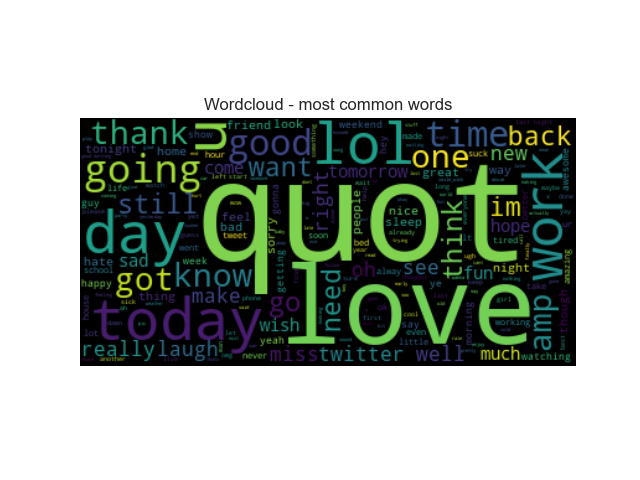
\includegraphics[width=\linewidth]{wordcloud}
\caption{\textbf{Wordcloud:} from figure we see the most common words in tweet. People often use quotes and words like day, today, love and word.}
\label{pic1}
\end{figure}

As can be seen from Figure \ref{pic2}, our classification problem is balanced. That is, the two classes are uniformly distributed. The next steps of preprocessing pipeline consists of the following:
\begin{enumerate}
	\item Remove non-ASCII characters.
	\item Remove links, hashtags, mentions and repetitive vowels (such as ``hahaa'').
	\item Replace laughing with a predefined word ``laugh''.
	\item Replace emojis with predefined combinations such as ``smile''.
	\item Switch to lower case.
	\item Filter stopwords.
	\item Tokenize words and turn them into appropriate form (depending on the algorithm).
\end{enumerate}

We also tried to improve evaluation metric scores with stemming words, fixing misspells, handling negations and removing retweets. However, these preprocessing techniques made the models overfit faster and effectively reduced evaluation metric scores. While, Naive Bayesian classifier was not really effected by those, LSTM and BERT performed worse. We assume that performance drop occured due to different pretraining in BERT and failing to find appropriate embeddings in LSTM with word embeddings. Rows with null values were dropped and finally, we used 80\% of data for training and the rest for testing our models.

\begin{figure}[hbt!]\centering
\centering
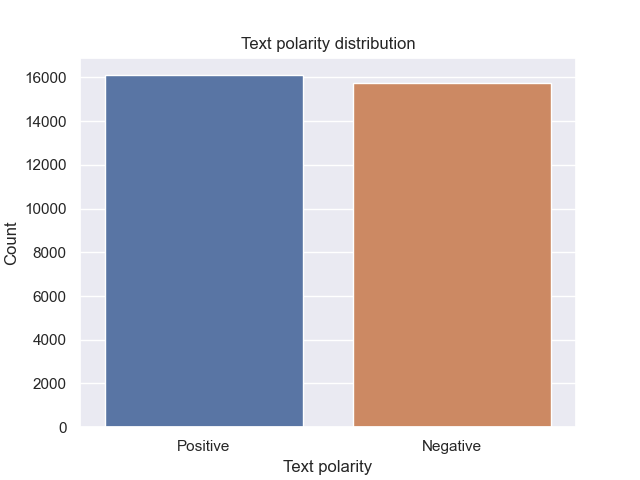
\includegraphics[width=\linewidth]{text-polarity-distr}
\caption{\textbf{Text polarity distribution: from figure we denote that text polarity is almost uniformly distributed. Both classes are representable. }}
\label{pic2}
\end{figure}

In Figure \ref{pic3}, we can see the distribution of tweet length after preprocessing. This later helpes us define parameters and model complexities in neural networks.

\begin{figure}[hbt!]\centering
\centering
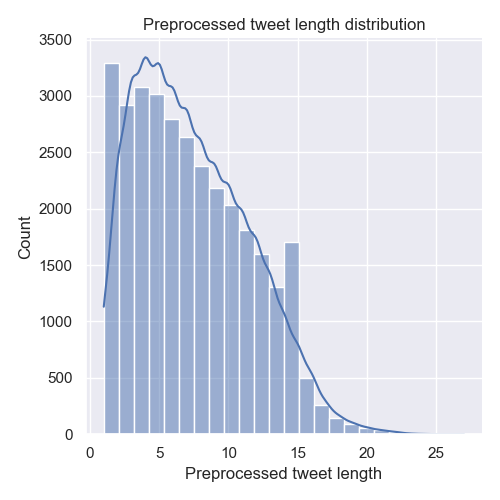
\includegraphics[width=\linewidth]{tweet-len-distr}
\caption{\textbf{Preprocessed tweet length distribution:} as can be seen from the figure, the distribution is right-skewed. This means that more tweets are short. The distribution does not have a long tail, which is why, we do not have to handle outliers in this situation.}
\label{pic3}
\end{figure}



\subsection{Naive Bayes}
Naive Bayesian classifier is one of the fastest and easiest methods that can also perform very well. The basic idea of this classifier is to find the probabilities of classes based on the input text. Textual data is passed to the model with word count vectors. With bigger datasets this model overfits, however, it tends to be used as the baseline model.

\subsection{LSTM}
As already mentioned, LSTM has been proven to be very succesful in sentiment analysis. We used the aforementioned bidirectional LSTM architecture with GloVe word embeddings instead of matrix of tokenized word encodings. We used GloVe with 200 dimensional representations. Next, we describe the architecture of the LSTM model in more detail:
\begin{enumerate}
	\item Model accepts a matrix of tokenized tweets padded to the pre-defined maximum length. This was set to 60 due to tweet length distribution.
	\item To decrease the chance of overfitting, we transform this matrix to a matrix of word embeddings and only use the top 4000 most common words.
	\item Learning rate is set to $5\mathrm{e}{-5}$ and we train the model for maximum 100 epochs. Early stopping is implemented if the model starts to overfit.
	\item The model consists of two bidirectional LSTM layers with dropout (once again, to prevent overfitting).
	\item In the end results are densed using ReLU activation function and on the last layer a sigmoid function.
	\item We use binary crossentropy loss function and Adam optimizer.
\end{enumerate}

Despite all the precautions we did against overfitting, the model performance still becomes too dependent on the training set after first few epochs as we can see in Figures \ref{pic4}, \ref{pic5}. 

\begin{figure}[hbt!]\centering
\centering
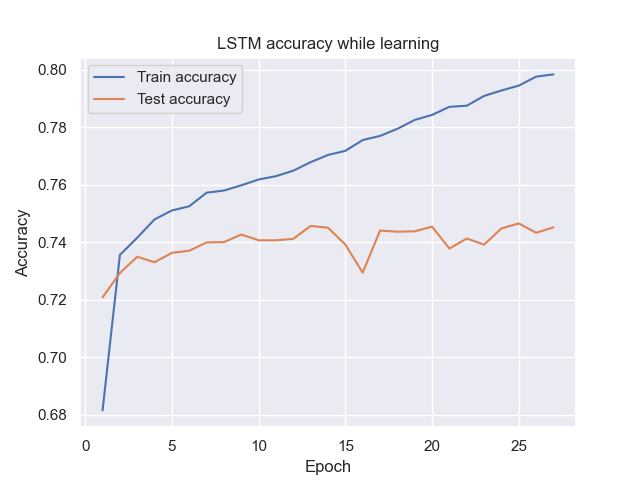
\includegraphics[width=\linewidth]{lstm-accuracy-27}
\caption{\textbf{LSTM accuracy:} in first few epochs accuracy is rising quickly. However, it becomes more or less constant in median after 5 or 10 epochs, while varying up and down.}
\label{pic4}
\end{figure}

\begin{figure}[hbt!]\centering
\centering
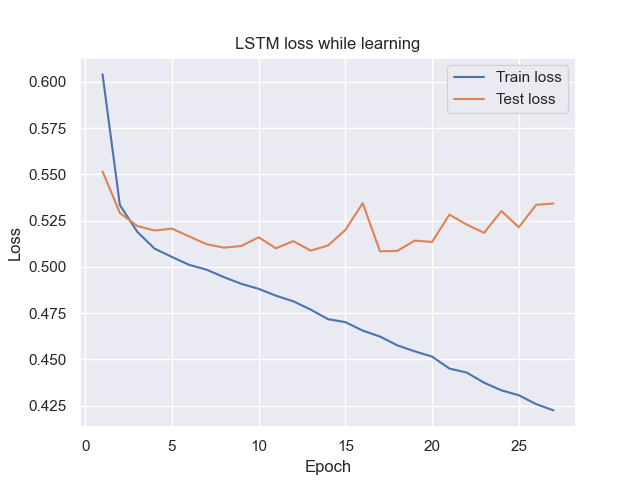
\includegraphics[width=\linewidth]{lstm-loss-27}
\caption{\textbf{LSTM loss:} in first few epochs loss is dropping quickly. However, it becomes more or less constant in median after 5 or 10 epochs, while varying up and down.}
\label{pic5}
\end{figure}

\subsection{BERT}


\subsection{Majority voting ensemble classifier}
Lastly, we explain the ensemble classifier that exploits the aforementioned three models and predicts the class with majority voting. With such ensemble method, we should get a more robust model. Evaluation metric scores could also be increased with such methods.

\section{Results}
Finally, we present results using the methodology that we described above. To better understand, how well our models generalize, we used a 10-fold cross validation in all the models. Using local resources with 6GB GPU, we managed to train 33 different models.

\begin{table*}
\centering
\begin{adjustbox}{width=0.8\textwidth}
\begin{tabular}{lllllllll}
\hline
\textbf{Algorithm}                                                                           & \multicolumn{2}{c}{\textbf{Accuracy}} & \multicolumn{2}{c}{\textbf{Precision}} & \multicolumn{2}{c}{\textbf{Recall}} & \multicolumn{2}{c}{\textbf{F1 score}} \\ \hline
\multicolumn{1}{l|}{}                                                                        & Train   & \multicolumn{1}{l|}{Test}   & Train   & \multicolumn{1}{l|}{Test}    & Train  & \multicolumn{1}{l|}{Test}  & Train             & Test              \\ \cline{2-9} 
\multicolumn{1}{l|}{\textbf{Naive Bayes}}                                                    & 0.855   & \multicolumn{1}{l|}{0.733}  & 0.855   & \multicolumn{1}{l|}{0.739}   & 0.857  & \multicolumn{1}{l|}{0.725} & 0.856             & 0.732             \\
\multicolumn{1}{l|}{\textbf{LSTM}}                                                           & 0.810   & \multicolumn{1}{l|}{0.745}  & 0.790   & \multicolumn{1}{l|}{0.730}   & 0.848  & \multicolumn{1}{l|}{0.781} & 0.818             & 0.755             \\
\multicolumn{1}{l|}{\textbf{BERT}}                                                           & 0.951   & \multicolumn{1}{l|}{0.775}  & 0.953   & \multicolumn{1}{l|}{0.783}   & 0.951  & \multicolumn{1}{l|}{0.763} & 0.952             & 0.773             \\
\multicolumn{1}{l|}{\textbf{\begin{tabular}[c]{@{}l@{}}Majority classifier\end{tabular}}} & 0.896   & \multicolumn{1}{l|}{0.768}  & 0.890   & \multicolumn{1}{l|}{0.765}   & 0.905  & \multicolumn{1}{l|}{0.776} & 0.897             & 0.771             \\ \hline
\end{tabular}
\end{adjustbox}
\vspace*{0.2cm}
\caption{}
\label{pic3}
\end{table*}


\begin{figure}[hbt!]\centering
\centering
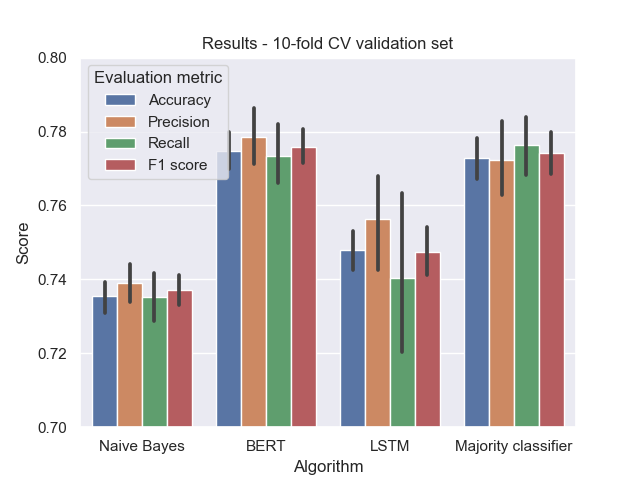
\includegraphics[width=\linewidth]{cv-test}
\caption{}
\label{pic6}
\end{figure}

\begin{figure}[hbt!]\centering
\centering
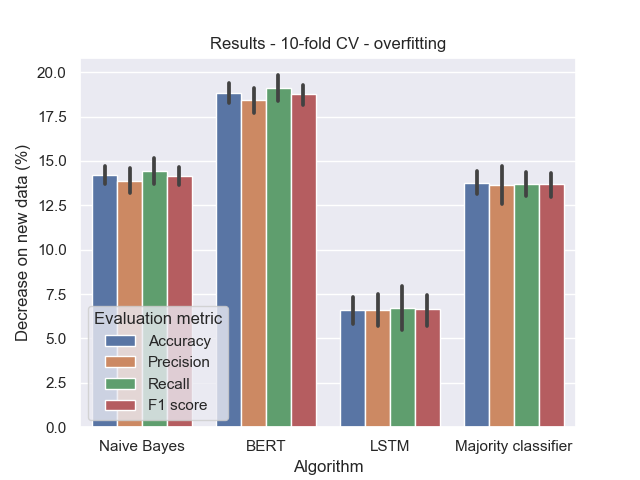
\includegraphics[width=\linewidth]{cv-overfitting}
\caption{}
\label{pic7}
\end{figure}


\section{Discussion}

\section{Conclusion}

% An example of a floating figure using the graphicx package.
% Note that \label must occur AFTER (or within) \caption.
% For figures, \caption should occur after the \includegraphics.
% Note that IEEEtran v1.7 and later has special internal code that
% is designed to preserve the operation of \label within \caption
% even when the captionsoff option is in effect. However, because
% of issues like this, it may be the safest practice to put all your
% \label just after \caption rather than within \caption{}.
%
% Reminder: the "draftcls" or "draftclsnofoot", not "draft", class
% option should be used if it is desired that the figures are to be
% displayed while in draft mode.
%
%\begin{figure}[!t]
%\centering
%\includegraphics[width=2.5in]{myfigure}
% where an .eps filename suffix will be assumed under latex, 
% and a .pdf suffix will be assumed for pdflatex; or what has been declared
% via \DeclareGraphicsExtensions.
%\caption{Simulation Results.}
%\label{fig_sim}
%\end{figure}

% Note that IEEE typically puts floats only at the top, even when this
% results in a large percentage of a column being occupied by floats.


% An example of a double column floating figure using two subfigures.
% (The subfig.sty package must be loaded for this to work.)
% The subfigure \label commands are set within each subfloat command,
% and the \label for the overall figure must come after \caption.
% \hfil is used as a separator to get equal spacing.
% Watch out that the combined width of all the subfigures on a 
% line do not exceed the text width or a line break will occur.
%
%\begin{figure*}[!t]
%\centering
%\subfloat[Case I]{\includegraphics[width=2.5in]{box}%
%\label{fig_first_case}}
%\hfil
%\subfloat[Case II]{\includegraphics[width=2.5in]{box}%
%\label{fig_second_case}}
%\caption{Simulation results.}
%\label{fig_sim}
%\end{figure*}
%
% Note that often IEEE papers with subfigures do not employ subfigure
% captions (using the optional argument to \subfloat[]), but instead will
% reference/describe all of them (a), (b), etc., within the main caption.


% An example of a floating table. Note that, for IEEE style tables, the 
% \caption command should come BEFORE the table. Table text will default to
% \footnotesize as IEEE normally uses this smaller font for tables.
% The \label must come after \caption as always.
%
%\begin{table}[!t]
%% increase table row spacing, adjust to taste
%\renewcommand{\arraystretch}{1.3}
% if using array.sty, it might be a good idea to tweak the value of
% \extrarowheight as needed to properly center the text within the cells
%\caption{An Example of a Table}
%\label{table_example}
%\centering
%% Some packages, such as MDW tools, offer better commands for making tables
%% than the plain LaTeX2e tabular which is used here.
%\begin{tabular}{|c||c|}
%\hline
%One & Two\\
%\hline
%Three & Four\\
%\hline
%\end{tabular}
%\end{table}


% Note that IEEE does not put floats in the very first column - or typically
% anywhere on the first page for that matter. Also, in-text middle ("here")
% positioning is not used. Most IEEE journals/conferences use top floats
% exclusively. Note that, LaTeX2e, unlike IEEE journals/conferences, places
% footnotes above bottom floats. This can be corrected via the \fnbelowfloat
% command of the stfloats package.



% conference papers do not normally have an appendix


% use section* for acknowledgement





% trigger a \newpage just before the given reference
% number - used to balance the columns on the last page
% adjust value as needed - may need to be readjusted if
% the document is modified later
%\IEEEtriggeratref{8}
% The "triggered" command can be changed if desired:
%\IEEEtriggercmd{\enlargethispage{-5in}}

% references section

% can use a bibliography generated by BibTeX as a .bbl file
% BibTeX documentation can be easily obtained at:
% http://www.ctan.org/tex-archive/biblio/bibtex/contrib/doc/
% The IEEEtran BibTeX style support page is at:
% http://www.michaelshell.org/tex/ieeetran/bibtex/
%\bibliographystyle{IEEEtran}
% argument is your BibTeX string definitions and bibliography database(s)
%\bibliography{IEEEabrv,../bib/paper}
%
% <OR> manually copy in the resultant .bbl file
% set second argument of \begin to the number of references
% (used to reserve space for the reference number labels box)
%\begin{thebibliography}{1}

%\bibitem{IEEEhowto:kopka}
%D.~Chamberlain et al., \emph{Application of Semi-Supervised Deep Learning to Lung Sound Analysis}.\hskip 1em plus
%  0.5em minus 0.4em\relax Harlow, England: Addison-Wesley, 1999.
%\end{thebibliography}

\bibliographystyle{IEEEtran}
\bibliography{bibfile}	




% that's all folks
\end{document}


